\documentclass[landscape,a4paper]{article}
% Minimal Font Size
\usepackage{lmodern}
\usepackage{scrextend}
\changefontsizes[10pt]{7pt}
% ----------------------------
\usepackage[utf8]{inputenc}
\usepackage[T1]{fontenc}
\usepackage[LY1,T1]{fontenc}
\usepackage{tikz}
\usetikzlibrary{shapes,positioning,arrows,fit,calc,graphs,graphs.standard}
\usepackage[nosf]{kpfonts}
\usepackage[t1]{sourcesanspro}
\usepackage{multicol}
\usepackage{wrapfig}
\usepackage[top=2mm,bottom=2mm,left=2mm,right=2mm]{geometry}
\usepackage[framemethod=tikz]{mdframed}
\usepackage{microtype}
\usepackage{pdfpages}
\usepackage{enumitem} % itemize without indentation
\usepackage{array} %table
\usepackage{lipsum}
\usepackage{multicol}
\usepackage{easytable}
\setlength{\columnseprule}{0.4pt} % lines between columns
\usepackage{listings} % https://en.wikibooks.org/wiki/LaTeX/Source_Code_Listings
\usepackage{color}
\usepackage{blkarray} %https://tex.stackexchange.com/questions/59517/label-rows-of-a-matrix-by-characters
\usepackage{graphicx} % Images in doccument
\usepackage{tabularx}
\graphicspath{ {./images/} }

% \titleformat{\subsubsection}
% {\normalfont\normalsize\bfseries}{\thesubsubsection}{1em}{}

% https://tex.stackexchange.com/questions/119866/whats-a-good-way-to-insert-very-few-lines-of-code
\definecolor{green}{rgb}{0,0.6,0}
\definecolor{codegray}{rgb}{0.5,0.5,0.5}
\definecolor{codepurple}{rgb}{0.58,0,0.82}
\definecolor{backcolour}{rgb}{0.95,0.95,0.92}
\definecolor{light_orange}{RGB}{221,117,56}
\definecolor{cyan}{RGB}{75,255,255}
\definecolor{magenta}{RGB}{255,0,255}
% https://tex.stackexchange.com/questions/401750/quick-and-short-command-for-coloring-one-word
\newcommand{\blue}[1]{\textcolor{blue}{#1}}
\newcommand{\green}[1]{\textcolor{green}{#1}}
\newcommand{\yellow}[1]{\textcolor{yellow}{#1}}
\newcommand{\red}[1]{\textcolor{red}{#1}}
\newcommand{\purple}[1]{\textcolor{purple}{#1}}
\newcommand{\cyan}[1]{\textcolor{cyan}{#1}}
\newcommand{\magenta}[1]{\textcolor{magenta}{#1}}

% size of titles https://tex.stackexchange.com/questions/59726/change-size-of-section-subsection-subsubsection-paragraph-and-subparagraph-ti
\usepackage{titlesec}
\titleformat{\section}
{\normalfont\large\bfseries}{\thesection}{1em}{}
\titleformat{\subsection}
{\normalfont\normalsize\bfseries}{\thesubsection}{1em}{}


% -- Titles ----------------------------------------------------------
\titleformat*{\section}{\scshape\large\bfseries\color{red}}
\titleformat*{\subsection}{\scshape\normalsize\bfseries\color{orange}}
\titleformat*{\subsubsection}{\scshape\small\bfseries\color{light_orange}}
% \titlespacing*{<command>}{<left>}{<before-sep>}{<after-sep>}
\titlespacing*{\section}{0pt}{0px}{0px}
\titlespacing*{\subsection}{0pt}{0px}{0px}
\titlespacing*{\subsubsection}{0pt}{0px}{0px}

\lstdefinestyle{mystyle}{
    backgroundcolor=\color{backcolour},   
    commentstyle=\color{codegreen},
    keywordstyle=\color{magenta},
    numberstyle=\tiny\color{codegray},
    stringstyle=\color{codepurple},
    basicstyle=\ttfamily\footnotesize,
    breakatwhitespace=false,         
    breaklines=true,                 
    captionpos=b,                    
    keepspaces=true,                 
    numbers=left,                    
    numbersep=5pt,                  
    showspaces=false,                
    showstringspaces=false,
    showtabs=false,                  
    tabsize=2
}
\lstset{style=mystyle}

\begin{document}
\begin{multicols*}{4}
    \section{Uvod v Umetno inteligenco}

\subsection{Turingov test}
Opazovalec po pogovru ne more lociti racunalnika od cloveka.\\
    \section{Strojno ucenje}


\subsection{Problemski prostor, ocenjevanje znanja}

\subsection{Evalviranje hipotez}
Pomembni kriteriji:
\begin{itemize}[leftmargin=*,labelindent=0pt,labelwidth=0pt,itemsep=0pt,parsep=0pt,topsep=0pt]
    \item \textbf{konsistentnost} hipotez z primeri (ucnimi)
    \item \textbf{splosnost} (tocnost za nevidene primere)
    \item \textbf{razumljivost} hipotez
\end{itemize}
Ocenjevanje uspesnosti pri klasifikaciji na podlagi njihove \textbf{tocnosti}:\\
TP - true positive, FP - false positive, FN - false negative, TN - true negative
$$\text{Klasifikacijska tocnost}=\frac{TP+TN}{TP+TN+FP+FN}=\frac{TP+TN}{N}$$
Napaka 1. tipa = FP, napaka 2. tipa = FN
$$\text{Obcutljivost/senzitivnost}=TPR=\frac{TP}{TP+FN}$$

\subsection{Gradnja odlocitvenih dreves}
\textbf{Informacijski prispevek} $\text{Gain(A)}=I-I_{res}(A)$, I=H(C)
$$I_{\text{res}}=-\sum_{v_i\in A}p_{v_i}\sum_c p(c|v_i)\log_2p(c|v_i)$$
Za koliko se entropija zmanjsa po delitvi z Atributom A.\\
\textbf{Razmerje inofrmacijskega prispevka atributa A}:\\ 
$\text{IGR(A)}=\frac{\text{Gain(A)}}{\text{H(A)}}$\\


\subsubsection{TDIDT (Top down induction decision tree) algoritem}
Pozresen algoritem, ki \textbf{lokalno} izbira najbolsi atribut.\\
- kratkoviden algoritem

\subsubsection{Binarizacija atributov}
Aleternativa za resevanje problematike z vecvrednostnimi atributi:\\
Primer: barve $\in$ {rdeca, rumena, zelena, modra}\\
Strategije, razbijemo v dve mnozici:\\
- {{rdeca}, {rumena, zelena, modra}}\\
- {{rdeca, rumena}, {zelena, modra}}\\
\textbf{Prednost}: manjse vejanje drevesa.



\subsection{Ucenje iz sumnih podatkov (rezanje)}
\green{tocnost t}...verjetnost pravilnosti klasifikacije\\
\green{napaka e} $\dots$ $1-t$\\
\green{relativna frekvenca} $p=\frac{n}{N}$\\
\green{m-ocena} $p=\frac{n + p_a * m}{N+m}$\\
$m \dots$ koliko zaupam apriorni verjetnosti\\
$p_a$ apriorna verjetnost (domenski ekspert lahko pove)\\
\green{Laplacova ocena verjetnosti} $p=\frac{n+1}{N+k}$\\
k...stevilo vseh moznih razredov\\
\subsubsection{REP (reduced error prunning)} 
Dela dobro ce imamo veliko rezalno mnozico.\\
Obicajno uporabljamo relativno frekvenco za ocenjevanje verjetnosti.\\
$G(v)=\#\text{napak}_T-\#\text{napak}_v$\\
$G(v)\geq 0 \Rightarrow$ rezemo podrevo\\
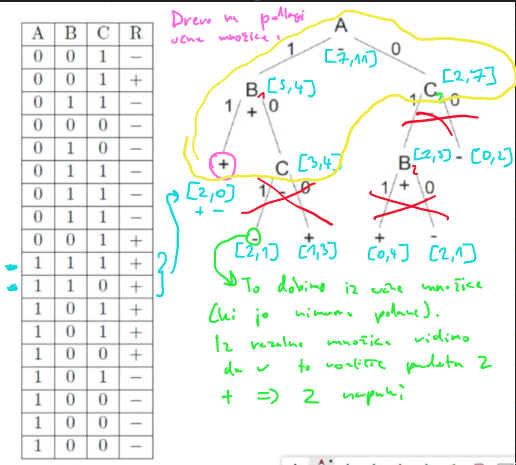
\includegraphics[width=6.5cm]{./images/rep.png}\\
$e(C)=3$\\
$e_T=2+3=5$\\
$G(C)=5-3=2\geq0 \rightarrow \text{rezemo}$
\subsubsection{MEP (Minimal Error Prunning)}
e...staticna napaka,E...vzvratna napaka,$e\leq E \rightarrow$ rezemo poddrevo\\
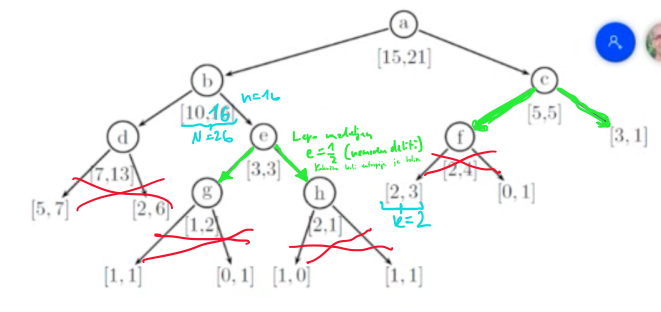
\includegraphics[width=6cm]{./images/mep.png}\\
(Laplace)\\
$e_L(d)=1-t=1-\frac{13+1}{20+2}=0.363$\\
$E_L(d)=12/20\cdot e_L(d_l) + 8/20\cdot e_L(d_d)= \frac{12}{20} \cdot(1-\frac{7+1}{12+2})+\frac{8}{20}(1-\frac{13+1}{20+2})$\\


\subsection{Ocenjevanje uspesnosti modelov}
\green{tocnost t} $\dots$ verjetnost pravilnosti klasifikacije\\
\green{Laplacova ocena verjetnosti} $p=\frac{n+1}{N+k}$\\
k...stevilo vseh moznih razredov\\
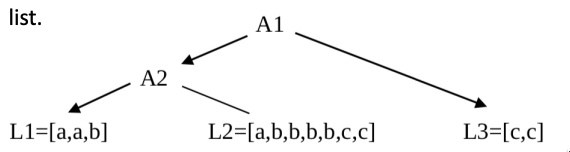
\includegraphics[width=6cm]{./images/drevo-laplace.png}\\
$t_{L1}=\frac{2+1}{3+3}=0.5$,
$t_{L2}=\frac{4+1}{7+3}=0.5$,
$t_{L3}=\frac{2+1}{2+3}=0.6$\\
tocnost drevesa: $t_D=3/12\cdot 0.5 + 7/12\cdot 0.5 + 2/12\cdot 0.6=0.5167$\\
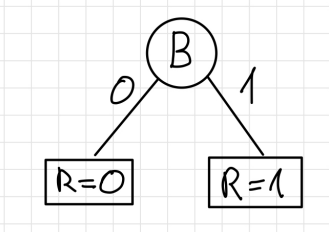
\includegraphics[width=6cm]{./images/klasifikacijska-napaka.png}\\
$e=1-(P(B=0)P(R=0|B=0)+P(B=1)P(R=1|B=1))$\\


\subsection{Obravnanva mankajocih atributov, navini Bayesov klasifikator}
\subsubsection{Naivni bayes}
Ce poznamo razred, kam klasificiramo ce nepoznamo atributov:
$$\text{Klasifikator: }\text{argmax}_{c\in C} P(c)\prod_{i=1}^n P(x_i|c)$$
$c\dots \text{razred}$, $x_i\dots \text{atributi}$\\
Verjetnost::
$$P(C=c|x_1,\dots,x_n)=\frac{P(C=c)P(X_1=x_i|C=c)P(X_2=x_j|C=c)\dots}{P(X_1=x_i)P(X_2=x_j)\dots}$$

\text{Primer moski}: $\text{visina}\geq175, \text{teza}\geq 65, \text{spol}=M$
$$
\begin{array}{|c|c|c|}
    \hline
    X\backslash Y   & \text{Razred A}      & \text{Razred B}\\
    \hline
    p_a           & P(A) = \frac{2}{3}    & P(B) = \frac{1}{3}\\
    \hline
    \text{spol}   & P(M|A) & P(M|B)\\
    \hline
    \text{visina} & P(V\geq 175|A) & P(V\geq 175 | B)\\
    \hline
    \text{teza} & P(T\geq 65|A) & P(T\geq 65| B)\\
    \hline
    P(y)\prod\limits_{i=1}^n P(x_i|y) & \dots & \dots\\
    \hline
\end{array}
$$

\subsubsection{Nomogragmi}
Ciljni razred $C=c_T$
$$X_{X_i=x_j}=\ln \left( \frac{P(X_i=x_j|C=c_T)}{P(X_i=x_j|C=\overline{c_T})} \right)$$

\subsection{K-najblizjih sosedov}
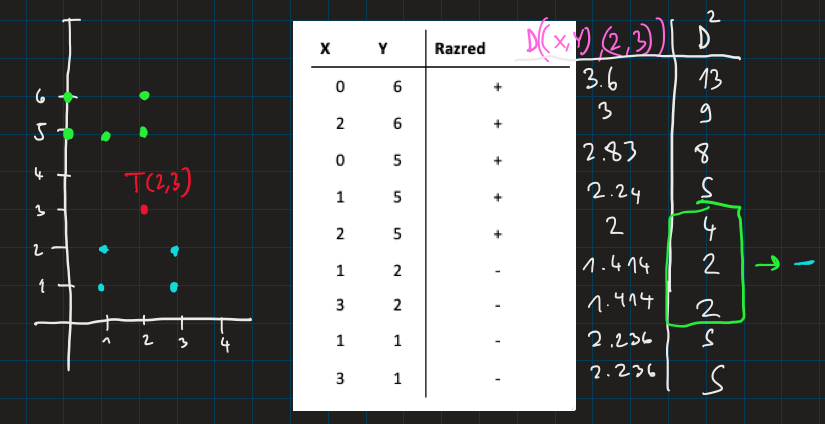
\includegraphics[width=6cm]{./images/knn.png}\\


\section{Vrste ucenja}
\subsection{Nadzorovano ucenje (supervised learning)}
\textbf{Ucni primeri so podani/oznaceni} kot \textbf{vrednosti vhodov in izhodov}.\\
$(\vec{x}_1,\vec{y}_1),(\vec{x}_2,\vec{y}_2),\dots,(\vec{x}_N,\vec{y}_N)$\\
$\vec{x}_i\dots$ atributi, $\vec{y}_i\dots$ ciljna spremenljivka\\
Locimo dve vrsti problemov:
% Create the list of problems with no margins
\begin{enumerate}[leftmargin=*,noitemsep,topsep=0pt,partopsep=0pt]
    \item \textbf{Klasifikacijski problemi} - $y_j$ \underline{diskretna} 
    \item \textbf{Regresijski problemi} - $y_j$ \underline{zvezna} 
\end{enumerate}

\subsubsection{Lokalno utezena regresija}
$$h(\vec{x}_?) = \frac{\sum\limits_{i=1}^k w_i\cdot f(\vec{x}_i)}{\sum\limits_{i=1}^k w_i}, \: w_i(d) ... \text{utez}$$
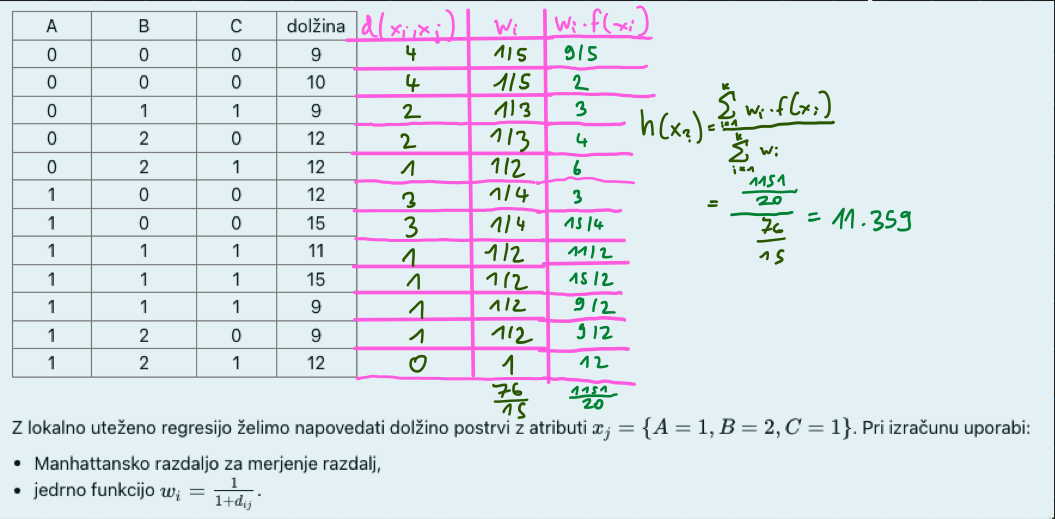
\includegraphics[width=7cm]{./images/lokalno-utezena-regresija.png}\\



\subsubsection{Regresijska drevesa}
Linearna regresija je poseben primer regresijskega drevesa.\\
V listih regresijskega drevesa vcasih napovemo kar povprecno vrednost.

\subsection{Nenadzorovano ucenje (unsupervised learning)}
\textbf{Ucni primeri niso oznaceni} (nimajo ciljne spremenljivke),
\textbf{ucimo se vzorcev v podatkih}, (npr. grucenje)

\subsubsection{Hierarhicno grucenje}
Poveze po podobnosti med primeri, primer zacne kot samostojna gruca, na koncu vsi primeri pripadajo eni gruci\\
\textbf{Dendrogram}: drevo, ki predstavlja grucenje.\\
\textbf{Single-linkage}: povezava med grucami je najkrajse razdalje med primeroma iz razlicnih gruc.\\
\textbf{Complete-linkage}: povezava med grucami je najdaljsa razdalja med primeroma iz razlicnih gruc.\\
\textbf{Average-linkage}: povezava med grucami je povprecna razdalja med primeroma iz razlicnih gruc.\\


\subsubsection{K-means}
1. V prostor dodamo k centroidov, ki predstavljajo gruce.\\
2. Izracunamo ketri centroid je najblizji vsakemu primeru.\\
3. Izracunamo nove centre gruc = $\frac{1}{|G|}\sum\limits_{i\in G} x_i$\\
4. Ponovimo korake 2 in 3 dokler se centri ne premaknejo.\\

\subsection{Spodbujevalno ucenje - reinforcement learning}
Inteligentni agent se uci iz zaporedja \textbf{nagrad} in \textbf{kazni}

\subsection{Ocenjevanje ucenja}

\subsubsection{Precno preverjanje}
Poseben primer \textbf{veckratnega ucenja} in testiranja\\
\textbf{k-kratno precno preverjanje}
\begin{itemize}[leftmargin=*,noitemsep,topsep=0pt,partopsep=0pt]
    \item celo ucno mnozico razbij na k disjunktnih podmnozic
    \item za vsako od k podmnozic:
    \begin{itemize}[leftmargin=*,noitemsep,topsep=0pt,partopsep=0pt]
        \item uporabi \textbf{mnozico} kot \textbf{testno mnozico}
        \item uporabi \textbf{preostalih k-1} mnozic kot \textbf{ucno mnozico}
    \end{itemize}
    \item povpreci dobljenih k ocen tocnosti v koncno oceno
\end{itemize}
Pri precnem preverjanju uporabimo vse podatke za testiranje in vse za ucenje\\
Metoda \textbf{leave one out} je poseben primer precnega preverjanja\\
Imamo dve hipotezi A in B. Izkase se, da A bolje napoveduje na ucnih podatkih
B pa na testnih. Potem je B verjetno boljsa hipoteza.

    \section{Preiskovanje}

\subsection{Neinformirani preiskovalni algoritmi}

\subsubsection{Iskanje v sirino}

\subsubsection{iskanje v globino}
Izboljsave (\textbf{Iskanje s sestopanjem, iterativno poglabljanje})

\subsubsection{iterativno poglabljanje}
problem gobinsko omejenega iskanja -> nastavitev meje l
Mejo l postopoma povecujemo za 1, dokler ne najdemo resitve.
% itemize without spacing
\begin{itemize}[noitemsep,topsep=0pt]
    \item \textbf{popolnost}: Da
    \item \textbf{optimalnost}: Da
    \item \textbf{casovna zahtevnost} $O(b^d)$
    \item \textbf{prostorska zahtevnost} $O(bd)$
\end{itemize}
Boljse od iskanja v globino/sirino
\subsubsection{dvosmerno iskanje}
Pozenemo vzporedni iskanji od zacetka do cilja in od cilja do zacetka.\\
\textbf{Implemenatcija dvosmernega iskanja}:
\begin{itemize}[noitemsep,topsep=0pt,leftmargin=*]
    \item ciljno vozlisce mora biti znano
    \item originalni problemski prostor preslikamo v dvosmerni prosto stanj
    E1, E2 dosegljiv iz E in S1,S2,S3 dosegljiv iz S
    (S,E) -> {(S1, E1), (S1,E2), (S2, E1), (S2, E2)...}
    Vozlisce (Si, Ei) je v dvosmernem prostur ciljo vozlisce ce velja E=S (soda dolzina na isto mesto pridemo iz obeh strani) ali S->E (liha pot sosednja)
\end{itemize}

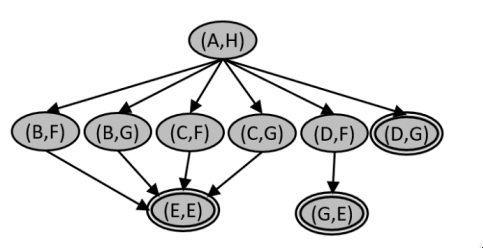
\includegraphics[width=\columnwidth]{images/dvosmerno-iskanje.png}

\subsection{Informirani preiskovalni algoritmi}
Ideja: preiskovanje usmerjamo z dodatnim znanjem \textbf{hevristiko} (ocenitvena funkcija za obetavnost vozlisca)\\
- \green{optimisticna/dopustna}: $\forall n: \bm{h(n) \leq h^*(n)}$ ($h^*$ je optimalna ocena)\\
- \green{optimalna}: $h(n) = h^*(n)$\\
- \green{pesimisticna}: $h(n) \geq h^*(n)$

\subsubsection{A*}
A* is informed version of \textbf{dijkstra} (uses heuristics and pq), ce h(dopustna)=\textbf{popolna in optimalna}\\
\textbf{Casovna zahtevnost} odvisna od hevristike: $E = (h^* - h)/h^*$, $O(b^{E \cdot d})$, b-stopnja vejanja, d-globina optimalne resitve\\ 
\textbf{Prostorska zahtevnost} \textbf{problem} (hrani vsa vozlisca v spominu)\\
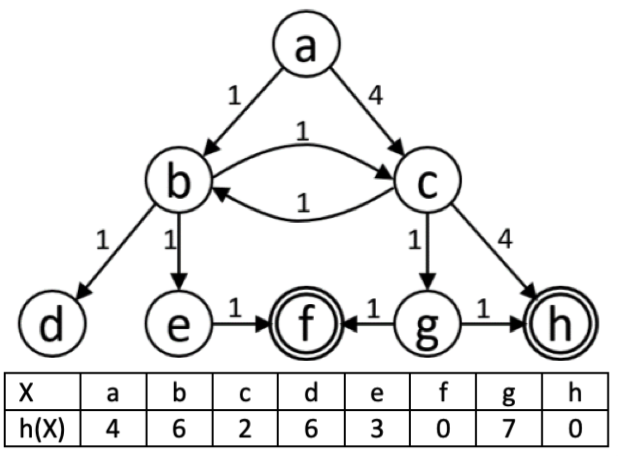
\includegraphics[width=\columnwidth]{./images/graf-a.png}\\
$f(n)=g(n)+h(n)$, g(n) cena do vozlisca, h(n) hevristika\\
Razvijamo dokler ne pridemo do ciljnega vozlisca\\
\begin{tabular}{c|c|c}
    Razvijano & Generirana & Priority Queue\\
    \hline
    / & a(4) & [] \\
    a & b(7) c(6) & $\left[ c(6), b(7)\right]$\\
    c & b'(11) g(12) h(8) & [b(7),h(8),b'(11),g(12)]\\
    b & c'(4) d(8) e(5) & [c'(4),e(5),h(8),d(8),b'(11),g(12)]\\
    \dots & \dots & \dots\\
    \magenta{f} & &
\end{tabular}

\subsubsection{IDA* (Iterative deepening A*)}
f(n) = g(n) + h(n), g(n)=cena poti do n\\
\begin{tabular}{c|c|c|c}
    Meja & Razvijano & Generirana & DFS (list)\\
    \hline
    0 & / & s(7) & /\\
    \hline
    7 & / & s(7) & s \\
      & s & a(8) b(7) c(7) & b, c\\
      & b & f(6) h(5) & f h c\\
      & f & g(7) h(9) i(11) & g h c\\
      & \underline{g} &  & 
\end{tabular}

\subsubsection{Kakovost hevristicnih funkcij}
Kakovost h ocenimo z \textbf{stevilom generiranih vozlisc} ter \textbf{efektivnim faktorjem vejanja} (N vozlisc je algoritem generiral da je na globini d nasel resitev)\\
Hocemo imeti dopustne hevristike s \textbf{cim visjimi vrednostmi} in \textbf{sprejelmjivo ceno} (casom izracuna)\\
Ce $h_2(n) \geq h_1(n), \forall n$ potem $h_2$ \textbf{dominira} $h_1$

\subsection{preiskovanje grafov AND/OR, nedeterministicno okolje}
Pomagajo resevati probleme z \textbf{dekompozicijo na manjse probleme}
Uporabnost:
\begin{itemize}[noitemsep,topsep=0pt,leftmargin=*]
    \item princip deli in vladaj
    \item iskanje v nedeterministicnih okoljih 
    \item igre med dvema nasprotnikoma s popolno informacijo (sah, dama)
    \item ekspertno resevanje problem
\end{itemize}
\subsubsection{AO*}
\begin{itemize}[noitemsep,topsep=0pt,leftmargin=*]
    \item posplositev A* na grafe AND/OR
    \item \textbf{popoln in optimalen} $\Leftrightarrow$ h(n) ne precenjuje dejanske cene do cilja
\end{itemize}
$F(N)$ ocena za usmerjanje preiskovanja, $H(N)$ dinamicna hevristicna ocena\\
Postopek:
\begin{enumerate}[noitemsep,topsep=0pt,leftmargin=*]
    \item Razvij najcenejse vozlisce
    \begin{itemize}[noitemsep,topsep=0pt,leftmargin=*]
        \item ce list in koncno (oznaci), preveri 3. korak, nadaljuj v 1.
        \item ce list in ni koncno (oznaci) vrednost vozlisca = $\infty$
    \end{itemize}
    \item Posodobi vse predhodnike
    \begin{itemize}[noitemsep,topsep=0pt,leftmargin=*]
        \item v AND starsih, cena starsa = $\sum$ sinov + povezava v
        \item v OR starsih, cena starsa = min(sinovi) + povezava v
    \end{itemize}
    \item Koncaj ko obstaja pot od zacetnega vozlisca, po kateri v AND vozliscih po vseh sinovih prides do cilja, v OR vozliscih v vsaj enem
\end{enumerate}
\subsubsection{algoritem MINIMAX}
$O(n^d)$
\subsubsection{Rezanje alfa-beta}
V najblsem primeru zmansa iz $O(b^{m \cdot d})$ na $O(b^{m \cdot d/2})$\\
\subsection{Lokalno preiskovalni algoritmi}
plezanje na hrib, simulirano ohlajanje, gen.algoritmi...
\subsubsection{Lokalno iskanje v snopu}
generiraj k nakljucnih zacetnih stanj\\
iz vsakegea generiraj sosede\\
izberi k najboljsih naslednikov\\
ponavljaj (iz maksimum stohasticno iskanje -> 1-verjetnost/sumvseh)

    \section{Planiranje}

\textbf{plan} zaporedje akcij, ki pripelje od zacetnega do koncnega stanja

\subsection{STRIPS}
Agentu opisemo svet in postavimo fizikalne omejitve.\\
Ne zagotovalja optimalne resitve, obravnavamo le en cilj naenkrat (ko ga dosezemo, se lahko ostali izgubijo) = Sussmanova anomalija\\
\green{Akcija} move(X, From, To)
\begin{itemize}[noitemsep,topsep=0pt,leftmargin=*]
    \item pogoj: \blue{cond}=[clr(X), on(X,F), clr(T)] $\rightarrow$ pogoji za izvajanje akcije,
    \item poz. ucinki: \blue{adds}=[on(X, T), clr(F)] $\rightarrow$ nova stanja,
    \item neg. ucinki: \blue{dels}=[on(X, F), clr(T)] $\rightarrow$ izbrisana stanja,
    \item omejitve: \blue{constr}=[F $\neq$ T, X$\neq$ F, X$\neq$ T, block(X)] $\rightarrow$ omejitve akcij (fizikalne omejitve),
\end{itemize}
\cyan{Algoritem}:
\begin{enumerate}[noitemsep,topsep=0pt,leftmargin=*]
    \item Izberi se neresen cilj iz mnozice CILJEV
    \item Izberi akcijo, ki izbrani cilj doda v stanje
    \item Omogoci izbrano akcijo (izpolni pogoje)
    \item Izvedi akcijo (ki izopolni najvec pogojev)
    \item Ce obstajajo nereseni cilji $\Rightarrow$ 1.
\end{enumerate}
\magenta{Primer dfs, zlaganje kock}

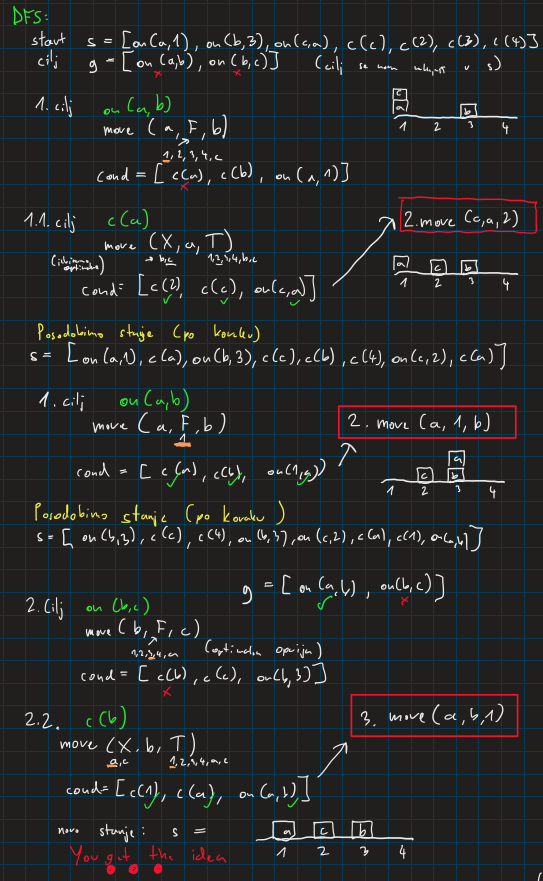
\includegraphics[trim={0cm 0cm 0cm 0cm},clip,width=6.5cm]{strips.png}



\subsection{PLANIRANJE Z REGRESIRANJEM CILJEV}
Resitev za sussmanovo anomalijo\\
Zacnemo v ciljih, regresiramo do zacetka ($G_i \subset S_0$):

\begin{enumerate}[noitemsep,topsep=0pt,leftmargin=*]
\item $G_{i+1} = G_i \cup \text{cond}(A) - \text{adds}(A)$
\item \blue{POGOJ}: $G_{i} \cap \text{dels}(A) = \emptyset$
\item Preveri da ni protislovja (npr. $G_{i+1} = \left[on(b,c), \dots, c(c) \dots\right]$)
\end{enumerate}

\green{PRIMER}:\\
$\rightarrow$ zactno\_stanje = [on(a,1), on(b,a), c(b), on(c,3), c(c)]\\
$\rightarrow$ hocemo da $\text{zacetno\_stanje} \subset G_i$
\begin{enumerate}[noitemsep,topsep=0pt,leftmargin=*,]
    \item $G_0$ = [on(a,b), on(b,c)]
    \begin{itemize}[noitemsep,topsep=0pt,leftmargin=0.5cm]
        \item \green{on(a,b)}: $A_0=move(a, From, b)$
        \item From = 1
        \item POGOJ: $G_0 \cap \text{dels}(A_0) = \emptyset \green{\checkmark}$
        \item $G_1$ = [on(a,b), on(b,c), c(a), c(b), on(a,1)]-[c(1), on(a,b)] $\green{\checkmark}$
    \end{itemize}
    \item $G_1=$[on(b,c),c(a),c(b),on(a,1)]
    \begin{itemize}[noitemsep,topsep=0pt,leftmargin=0.5cm]
        \item \green{c(a)}: $A_1=move(X, a, To)$
        \item X = c, To = 2
        \item POGOJ: $G_1 \cap \text{dels}(A_1) = \emptyset \green{\checkmark}$
        \item $G_2$ = [\underline{on(b,c)},c(a),c(b),on(a,1),\underline{c(c)},c(2),on(c,a)]\\ -[c(a), on(c,2)] \xmark (protislovje)
        \item \green{on(b,c)}: $A_2=move(b, From, c)$
        \item From = 3
        \item POGOJ: $G_2 \cap \text{dels}(A_2) = \emptyset \green{\checkmark}$
        \item $G_2$ = [on(b,c),c(a),c(b),on(a,1),c(c),c(b),on(b,3)] \cmark
    \end{itemize}
    \item $G_2$ = ...     
\end{enumerate}
\subsection{RAZPOREJANJE OPRAVIL}


    \section{Sklepanje}
\subsection{Bayesovske mreze}
Baye. mreza = Usmerjen graf, kjer so podane zahtevane verjetnosti:
\begin{itemize}[leftmargin=*,topsep=0pt,noitemsep]
    \item Za vozlisca \textbf{brez starsev} verjetnosti $P(v_i)$
    \item Za vozlisca z \textbf{starsi} pogojne verjetnosti vseh kombinacij starsev
\end{itemize}
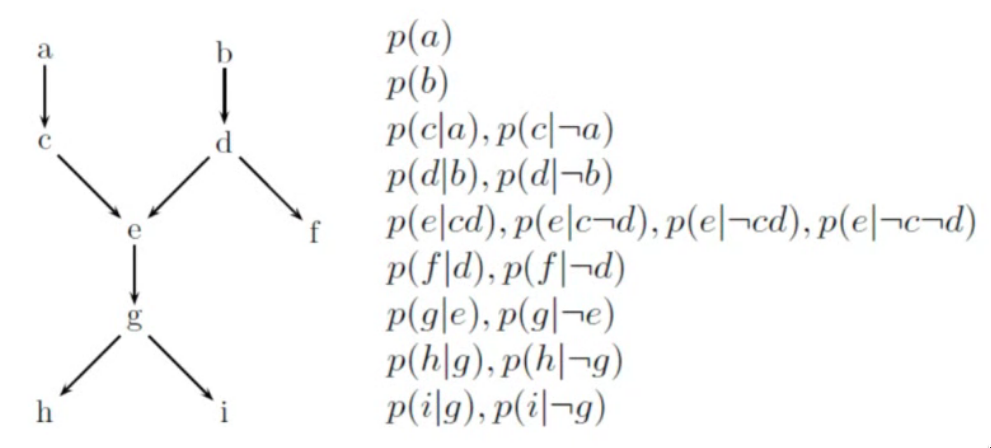
\includegraphics[width=6cm]{images/bayesovska_mreza.png}
Pravila verjetnostnega sklepanja:
\begin{enumerate}[leftmargin=*,topsep=0pt,noitemsep]
    \item \textbf{Konjunkcija}: $P(X_1 X_2 \mid C) = P(X_1 \mid C) P(X_2 \mid X_1C)$
        \begin{itemize}[leftmargin=*,topsep=0pt,noitemsep]
            \item $P(A_1\cap\dots\cap A_n) = \prod\limits_{k=1}^n P\left(A_k\mid \bigcap\limits_{j=1}^{k-1} A_j\right)$ 
        \end{itemize} 
    \item \textbf{Gotov dogodek}: $P(X \mid \dots X \dots) = 1$
    \item \textbf{Nemogoc dogodek}: $P(X\mid \dots \overline{X} \dots) = 0$
    \item \textbf{Negacija}: $P(\overline{X} \mid C) = 1 - P(X \mid C)$
    \item Ce je Y naslednik od X in je Y vsebovan v pogojnem delu: $P(X\mid YC) = P(X\mid C) \cdot \frac{P(Y\mid XC)}{P(Y\mid C)}$
    \item Ce pogojni del ne vsebuje naslednika od X:
        \begin{enumerate}[leftmargin=0.1cm,noitemsep,topsep=0pt,label=(\alph*)]
            \item ce X \textbf{nima} starsev: $P(X\mid C) = P(X)$, P(X) je podan
            \item ce \textbf{ima} X starse S: $P(X\mid C) = \sum_{S\in P_X} P(X \mid S)P(S\mid C)$
        \end{enumerate}
    \item Iz 6b zgoraj: $P(i \mid gc) = P(i \mid g)$
\end{enumerate}
\subsection{Ovojnica Markova}
X je \textbf{neodvisno} od vseh ostalih $\Leftrightarrow$ podani \textbf{starsi}, \textbf{otroci} in \textbf{starsi otrok}\\
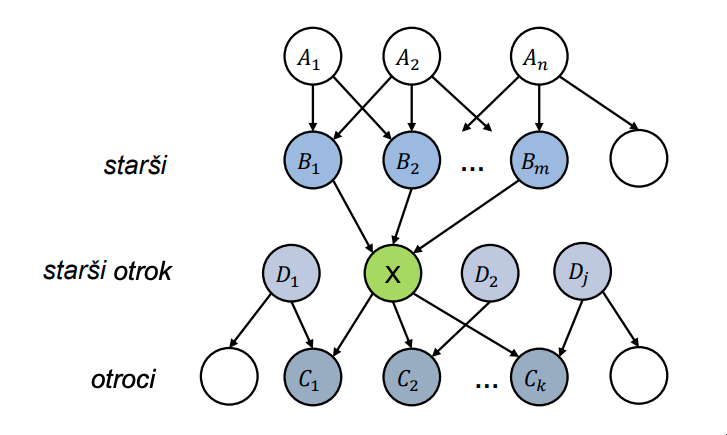
\includegraphics[width=3cm]{images/ovojnica-markova.png}
\subsection{D-locevanje}
A in B v mrezi sta \textbf{neodvisni} $\Leftrightarrow$ obstaja mnozica vozlisc E, ki d-locuje A in B, potem sledi:  (\green{$P(A|EB)=P(A|E)$})\\
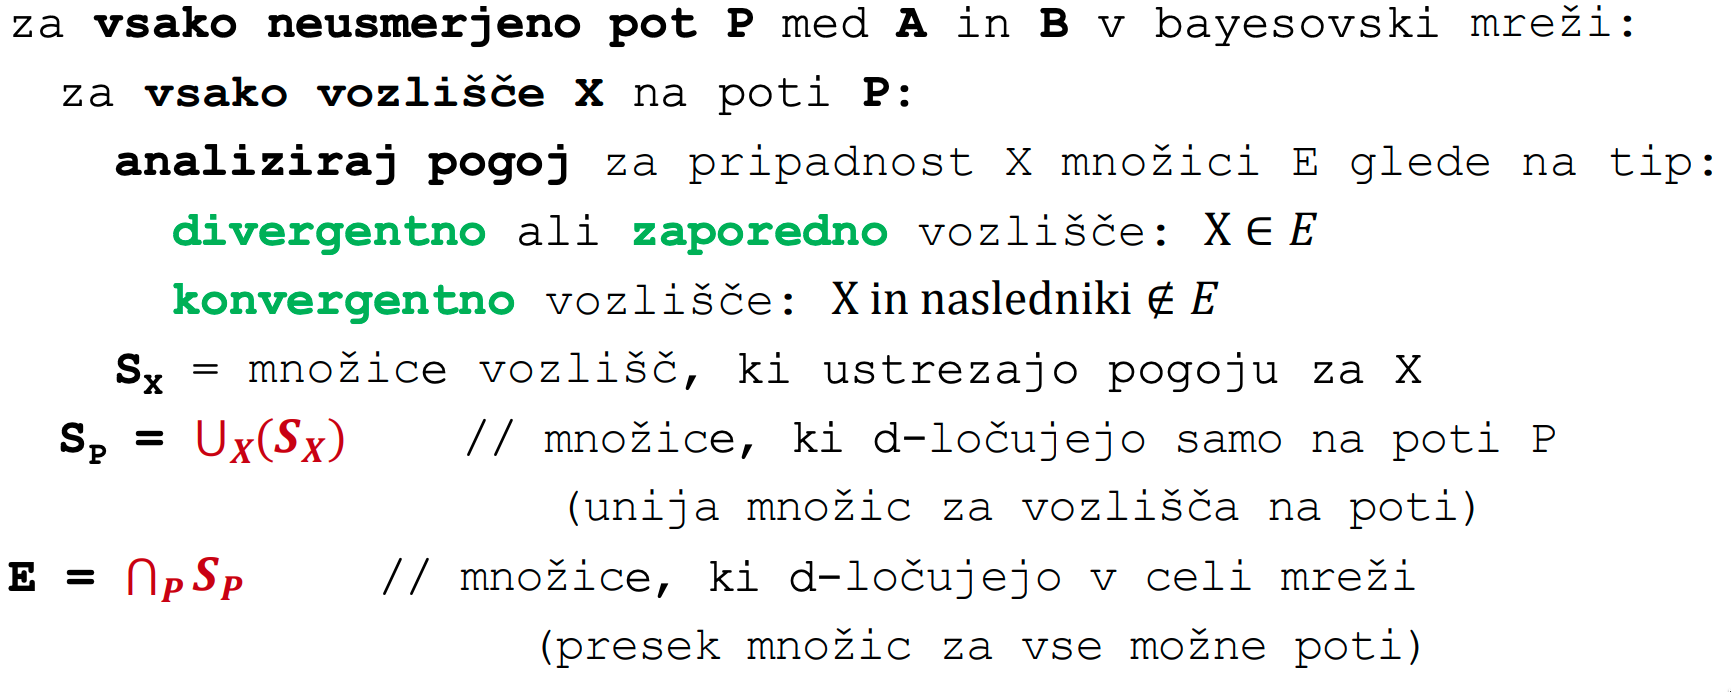
\includegraphics[width=6.5cm]{images/d-locevanje-algoritem.png}
\includegraphics*[width=7cm]{images/d-locevanje-nacini.png}
\red{! pri konvergentnem izlocimo tudi vse naslednike X}\\
Primer d-locevanje vozlisc c in d\\
\includegraphics*[width=6cm]{images/primer-d-locevanje.png}\\
$\rightarrow$ P(d|c\blue{a})=P(d|a), P(d|c\blue{b})=P(d|b), P(d|c\blue{ab})=P(d|ab),\\
P(d|c\blue{be})=P(d|be),P(d|c\blue{abe})=P(d|abe)
\subsection{I-ekvivalentnost}
Mrezi sta \green{I-ekvivalentni} ce imate \textbf{enako strukturo} (ob ignoriranju usmerjenosti povezav) in \textbf{ista konvergentna vozlisca}:\\
\includegraphics*[width=7cm]{./images/i-ekvivalentnost.png}
\end{multicols*}
\end{document}
